\documentclass[11pt]{article}
\usepackage{geometry} % Pour passer au format A4
\geometry{hmargin=1cm, vmargin=1cm} % 

% Page et encodage
\usepackage[T1]{fontenc} % Use 8-bit encoding that has 256 glyphs
\usepackage[english,french]{babel} % Français et anglais
\usepackage[utf8]{inputenc} 

\usepackage{lmodern}
\setlength\parindent{0pt}

% Graphiques
\usepackage{graphicx,float,grffile}

% Maths et divers
\usepackage{amsmath,amsfonts,amssymb,amsthm,verbatim}
\usepackage{multicol,enumitem,url,eurosym,gensymb}

% Sections
\usepackage{sectsty} % Allows customizing section commands
\allsectionsfont{\centering \normalfont\scshape}

% Tête et pied de page

\usepackage{fancyhdr} 
\pagestyle{fancyplain} 

\fancyhead{} % No page header
\fancyfoot{}

\renewcommand{\headrulewidth}{0pt} % Remove header underlines
\renewcommand{\footrulewidth}{0pt} % Remove footer underlines

\newcommand{\horrule}[1]{\rule{\linewidth}{#1}} % Create horizontal rule command with 1 argument of height

\newcommand{\tempsexo}[1]{\textit{\textbf{(#1)}}}
%----------------------------------------------------------------------------------------
%   Début du document
%----------------------------------------------------------------------------------------

\begin{document}

%----------------------------------------------------------------------------------------
% RE-DEFINITION
%----------------------------------------------------------------------------------------
% MATHS
%-----------

\newtheorem{Definition}{Définition}
\newtheorem{Theorem}{Théorème}
\newtheorem{Proposition}{Propriété}
\newtheorem{Exo}{Éxercice}

% MATHS
%-----------
\renewcommand{\labelitemi}{$\bullet$}
\renewcommand{\labelitemii}{$\circ$}
%----------------------------------------------------------------------------------------
%   Titre
%----------------------------------------------------------------------------------------

\setlength{\columnseprule}{1pt}

\section{S1 : Correction - Semaine du 16/03 au 22/03}

\subsection{Travail sur le chapitre - Fonctions linéaires}

\Exo{p122 ex1}\\
On considère la fonction f telle que $f(x) = -5x$

\begin{multicols}{3}
\begin{enumerate}
    \item[a.] 6
    \begin{align*}
        f(x) &= -5x \\
        f(6) &= -5 \times 6 \\
        f(6) &= -30    
    \end{align*}\columnbreak

    \item[b.] -1
    \begin{align*}
        f(x) &= -5x \\
        f(-1) &= -5 \times -1 \\
        f(-1) &= 5       
    \end{align*}\columnbreak

    \item[c.] -3
    \begin{align*}
        f(x) &= -5x \\
        f(-3) &= -5 \times -3 \\
        f(-3) &= 15       
    \end{align*}

\end{enumerate}
 \end{multicols}

\begin{multicols}{2}
\begin{enumerate}
     \item[d.] $\dfrac{6}{25}$
    \begin{align*}
        f(x) &= -5x \\
        f(\dfrac{6}{25}) &= -5 \times \dfrac{6}{25} \\
        f(\dfrac{6}{25}) &= \dfrac{-6}{5}       
    \end{align*}\columnbreak

     \item[e.] $\dfrac{-3}{7}$
    \begin{align*}
        f(x) &= -5x \\
        f(\dfrac{-3}{7}) &= -5 \times \dfrac{-3}{7} \\
        f(\dfrac{-3}{7}) &= \dfrac{15}{7}      
    \end{align*}                  
\end{enumerate}
\end{multicols}
Remarque : C'est également une bonne occasion pour utiliser la touche / fonction CALC de sa calculatrice.


\Exo{p122 ex3} \\
Les fonctions suivantes sont-elles des fonctions linéaires.
\begin{enumerate}
    \item[a.] $f(x) = 4x$ : \textbf{OUI}, on a bien un coefficient ($4$) qui multiplie x et rien d'autre. 
    \item[b.] $g(x) = 5 + x$ : \textbf{NON}, on a bien un coefficient ($1$) qui multiplie x MAIS on lui ajoute un autre nombre ($5+$).
    \item[c.] $h(x) = 3x - 5$ : \textbf{NON}, on a bien un coefficient ($3$) qui multiplie x MAIS on lui enlève un autre nombre ($-5$).
    \item[d.] $k(x) = \dfrac{3}{7}x$ : \textbf{OUI,} on a bien un coefficient ($\dfrac{3}{7}$) qui multiplie x et rien d'autre. 
\end{enumerate}

\Exo{p122 ex4} \\
\begin{minipage}[t]{0.3\textwidth}
  \begin{figure}[H]
        \centering
        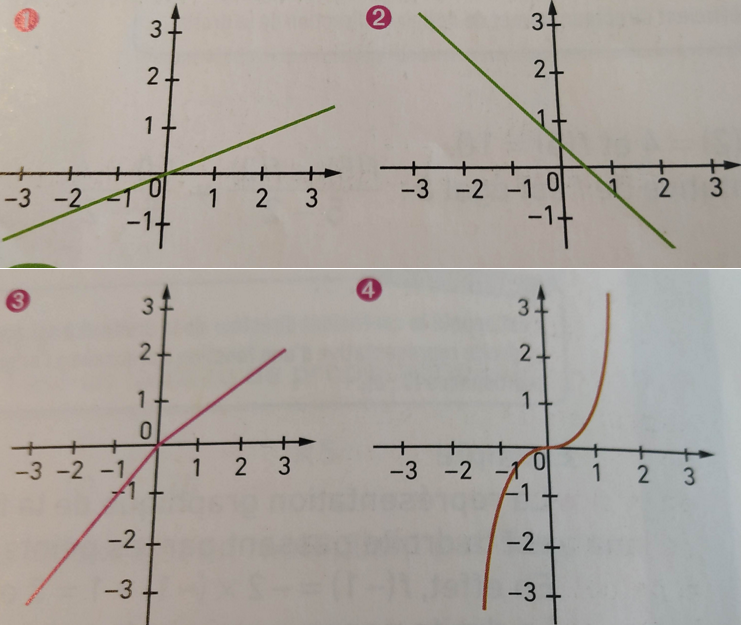
\includegraphics[width=0.9\linewidth]{_continuite/sources/s1-p122ex4.png}
  \end{figure}
\end{minipage}
\begin{minipage}[t]{0.7\textwidth}
Les fonctions suivantes sont-elles des fonctions linéaires.
\begin{enumerate}
    \item[1.] \textbf{OUI} : La représentation graphique est une droite qui passe par l'origine.
    \item[2.] \textbf{NON} : La représentation graphique est une droite mais ne passe pas par l'origine.
    \item[3.] \textbf{NON} : La représentation graphique passe par l'origine mais n'est pas UNE droite.
    \item[4.] \textbf{NON} : La représentation graphique passe par l'origine mais n'est pas une droite.
\end{enumerate}
\end{minipage}

\newpage
\Exo{p133 ex79} \\

\begin{enumerate}
    \item[1.] On calcule pour les formules. 
    \begin{multicols}{2}
    Tarif miniplouf : 7 entrées. \\
    $7 \times 6 = 42 $

    Tarif megaplouf : 1 carte et 7 entrées. \\
    $25 + 7 \times 3,5 = 49,5$ \\
    Pour 7 entrées, le tarif le plus intéressant est miniplouf. (42 \euro) \columnbreak

    Tarif miniplouf : 15 entrées. \\
    $15 \times 6 = 90 $

    Tarif megaplouf : 1 carte et 15 entrées. \\
    $25 + 15 \times 3,5 = 77,5$\\
    Pour 15 entrées, le tarif le plus intéressant est megaplouf. (77,5 \euro) 
    \end{multicols}
    \item[2.] On note x le nombre d'entrées.
     \begin{enumerate}
        \item[2a.]
        \begin{minipage}[t]{0.4\textwidth}
        Miniplouf, on paie 6\euro~ l'entrée. \\
        $f(x) = 6 \times x$ \\
        $f(x) = 6x$ \\
        \end{minipage}
        \begin{minipage}[t]{0.6\textwidth}        
        Megaplouf, on achète une carte puis on paie 3,5\euro~ l'entrée. \\
        $g(x) = 25  + 3.5 \times x$ \\
        $g(x) = 3.5x + 25$
\end{minipage}
        \item[2b.] La fonction $f$ est une fonction linéaire. La fonction g est une fonction affine.
    \end{enumerate}
    \item[3.]
    \begin{figure}[H]
        \centering
        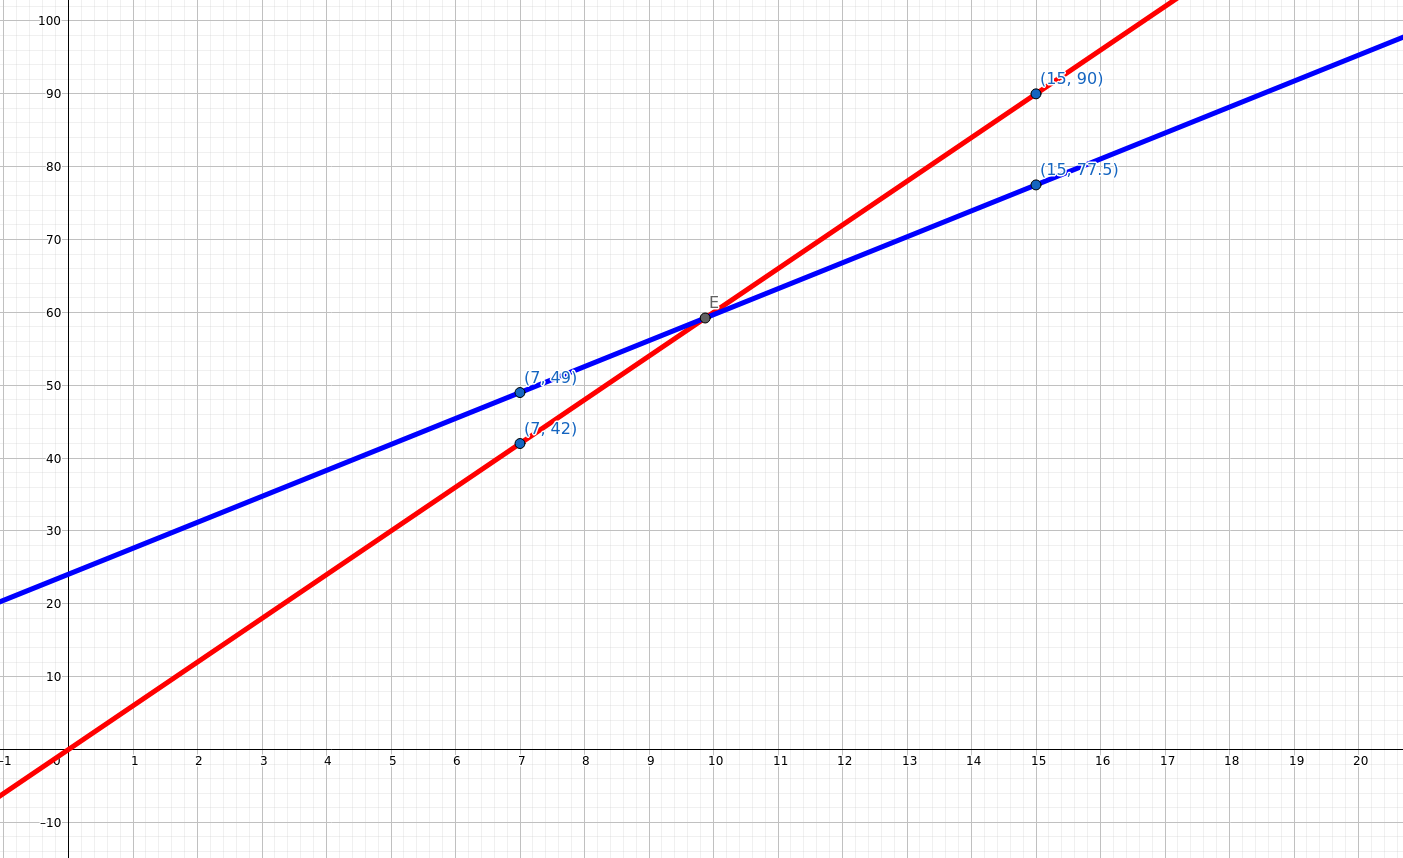
\includegraphics[width=0.9\linewidth]{_continuite/sources/s1-p133ex79.png}
    \end{figure}
    \item[4.] Graphiquement, on trouve que le tarif megaplouf devient plus intéressant à partir de 10 entrées. 
    \item[5.] On cherche x, le nombre d'entrées tel que les tarifs mégaplouf et miniplouf soient égaux.
    \begin{align*} 
        f(x) &= g(x) \\
         6x  &= 3.5x + 25 \\
         6x - 3.5x &= 25 \\
         2.5x &= 25 \\
         x &= \frac{25}{2.5} \\
         x &= 10
    \end{align*}
    Les tarifs miniplouf et megaplouf sont identiques pour 10 entrées. 

\end{enumerate}


\end{document}